\documentclass[xcolor=pdftex,dvipsnames,table,mathserif,aspectratio=169]{beamer}
\usetheme{default}
\usetheme{metropolis}
\usepackage{mathtools}
\setbeamersize{text margin left=.3in,text margin right=.3in} 

\DeclarePairedDelimiter\abs{\lvert}{\rvert}%
\DeclarePairedDelimiter\norm{\lVert}{\rVert}%

\usepackage[english]{babel}
\usepackage{pgf,pgfarrows,pgfnodes,pgfautomata,pgfheaps}
\usepackage{amsmath,amssymb,setspace,centernot}
\usepackage[latin1]{inputenc}
\usepackage{pgf,tikz}
\usepackage[T1]{fontenc}
\usepackage{relsize}
\usepackage{pdfpages}
\usepackage[absolute,overlay]{textpos} 


\newenvironment{reference}[2]{% 
  \begin{textblock*}{\textwidth}(#1,#2) 
      \footnotesize\it\bgroup\color{red!50!black}}{\egroup\end{textblock*}} 

\DeclareMathSizes{10}{10}{6}{6} 

\begin{document}
\title{$k$-Means and Grouped FE}
\author{Chris Conlon}
\institute{Applied Econometrics II}
\date{\today}

\frame{\titlepage}


\begin{frame}
\frametitle{Reading}
\begin{itemize}
\item Chapters 14 of \textit{Elements of Statistical Learning}
\item Bonhomme, Lamadon and Manresa
\begin{itemize}
\item A Distributional Framework for Matched Employer Employee Data (Econometrica 2020)
\item Discretizing Unobserved Heterogeneity (2021)
\end{itemize}
\end{itemize}
\end{frame}


\begin{frame}{$k$-means Clustering}
Idea: I have a matrix of data $\mathbf{X}$ ($N \times M$). 
\begin{itemize}
\item We are going to take the rows of $X$ and assign them to $K$ groups.
\begin{itemize}
\item Groups are mutually exclusive and exhaustive.
\end{itemize}
\item Goal: minimize residual variance:
\begin{align*}
\min_{\mu} \min_{k(i)} \sum_{i=1}^N \sum_{k=1}^K || \mathbf{x_i} - \mu_{k(i)} ||^2
\end{align*}
\item Choose both
\begin{itemize}
\item Assignment of each row to a group $k(i)$
\item Mean of each group $\mu_k$.
\end{itemize}
\end{itemize}
\end{frame}


\begin{frame}{$k$-means Clustering}
How does it work?
\begin{itemize}
\item Mean-Variance tradeoff
\begin{itemize}
\item More clusters: less bias, higher variance
\item Fewer clusters: more bias, less variance.
\end{itemize}
\item Naive idea: alternate between minimum distance to assign groups and recompute mean of group.
\item Honestly this is a difficult problem for the computer to solve ($NP$-hard).
\item You don't want to implement it on your own.
\item Use a canned routine.
  \item Choice of distance metric matters: Euclidean $L_2$, Mahalanobis (Covariance), Manhattan/Taxicab $L_1$.
\end{itemize}
\end{frame}

\begin{frame}[fragile]{How to choose $K$?}

\begin{columns}
\begin{column}{0.5\textwidth}
  \begin{itemize}
\item Tune with OOS MSE to choose $K$ via cross-validation
\item Most people use ``elbow method'' on the right.
\item See \url{https://www.datanovia.com/en/lessons/determining-the-optimal-number-of-clusters-3-must-know-methods/}
  \end{itemize}
  \centering
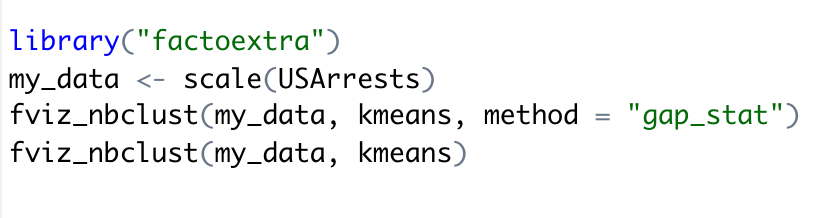
\includegraphics[height=0.2\textheight]{./resources/k_means_code.png}
\end{column}
\begin{column}{0.5\textwidth}  %%<--- here
    \begin{center}
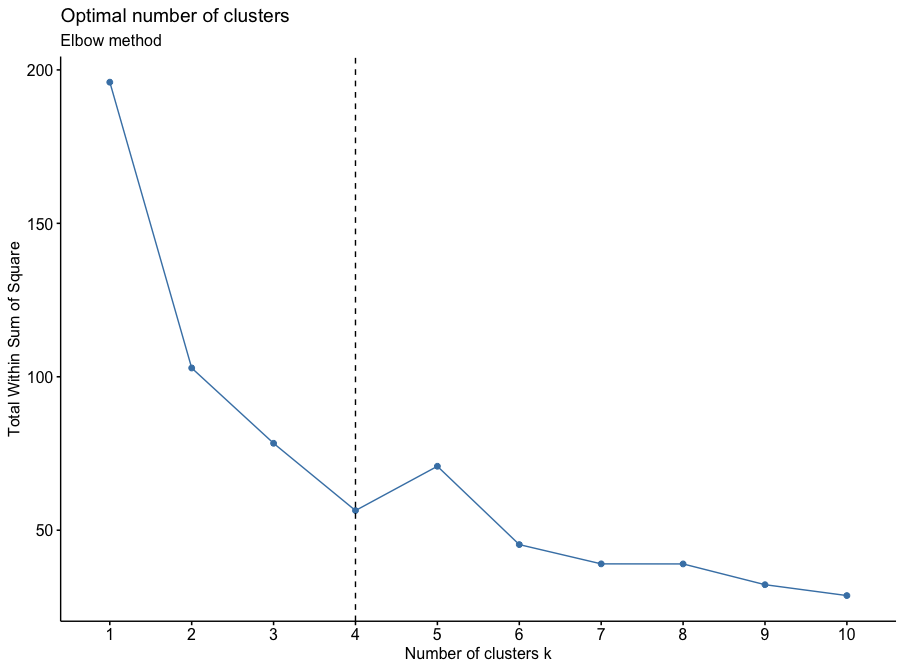
\includegraphics[height=0.5\textwidth]{./resources/k_means_fit1.png}\\
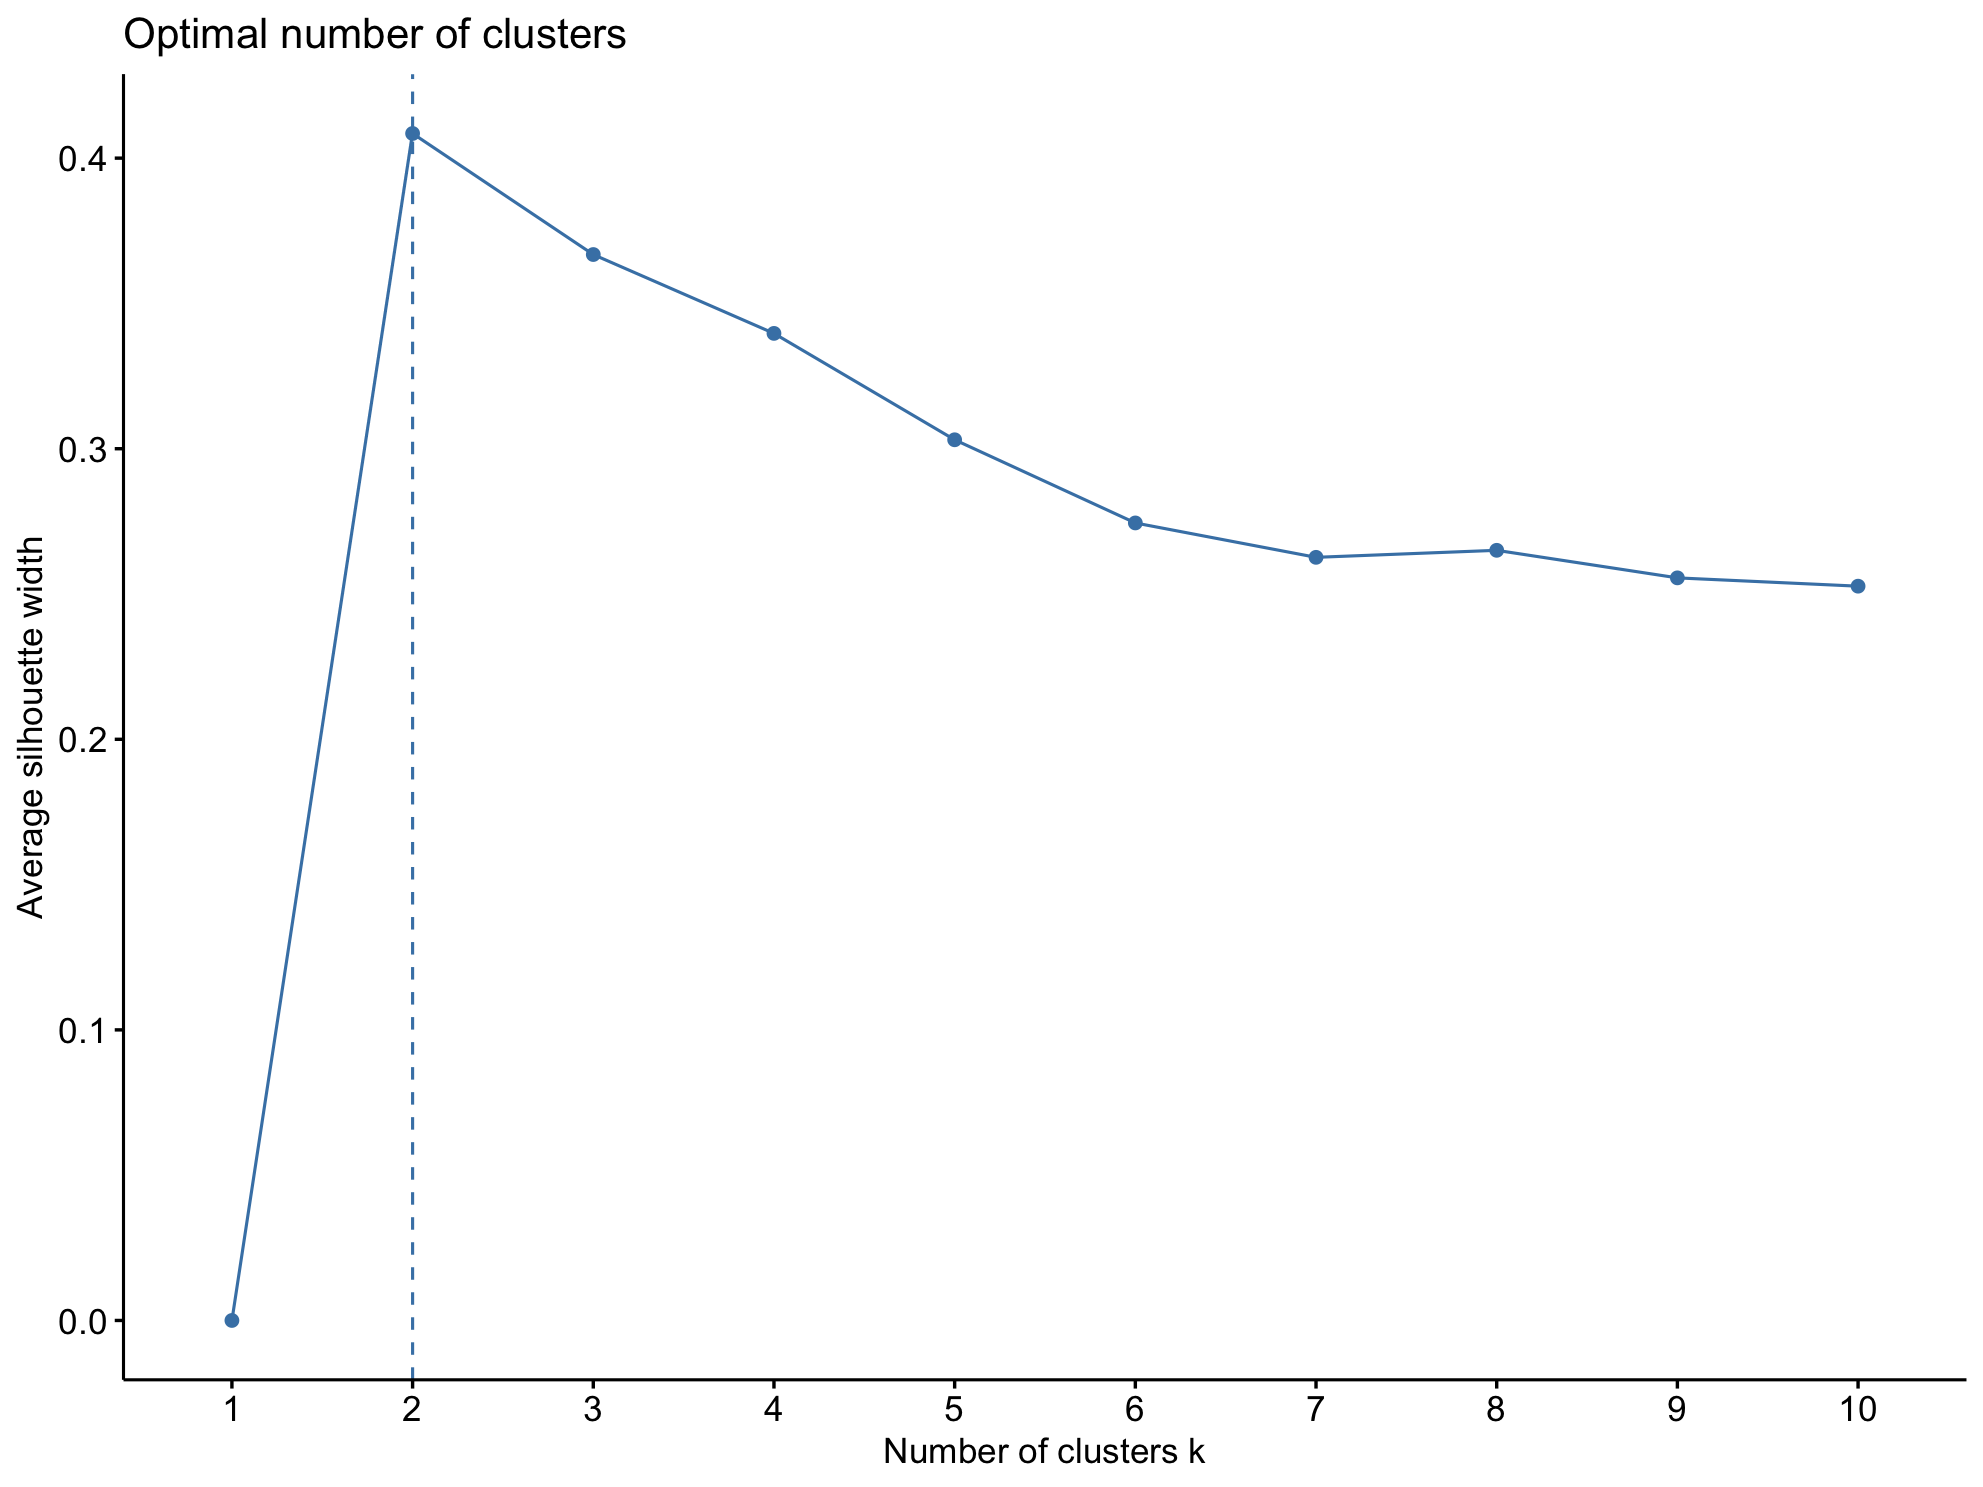
\includegraphics[width=0.7\textwidth]{./resources/k_means_fit2.png}\\
     \end{center}
\end{column}
\end{columns}

\end{frame}



\begin{frame}{Not as easy as it looks (figure from \texttt{scikit-learn})}

\begin{columns}
\begin{column}{0.5\textwidth}
  \begin{itemize}
\item Assumes that variance is essentially \alert{spherical} so standardize inputs first!
\item Rotations of space (e.g. PCA) will change the answer!
\item Scaling of the space (e.g. taking $\log(X)$) will change the answer!
\item Choosing wrong number of clusters $K$ is a bad idea.
  \end{itemize}
\end{column}
\begin{column}{0.5\textwidth}  %%<--- here
    \begin{center}
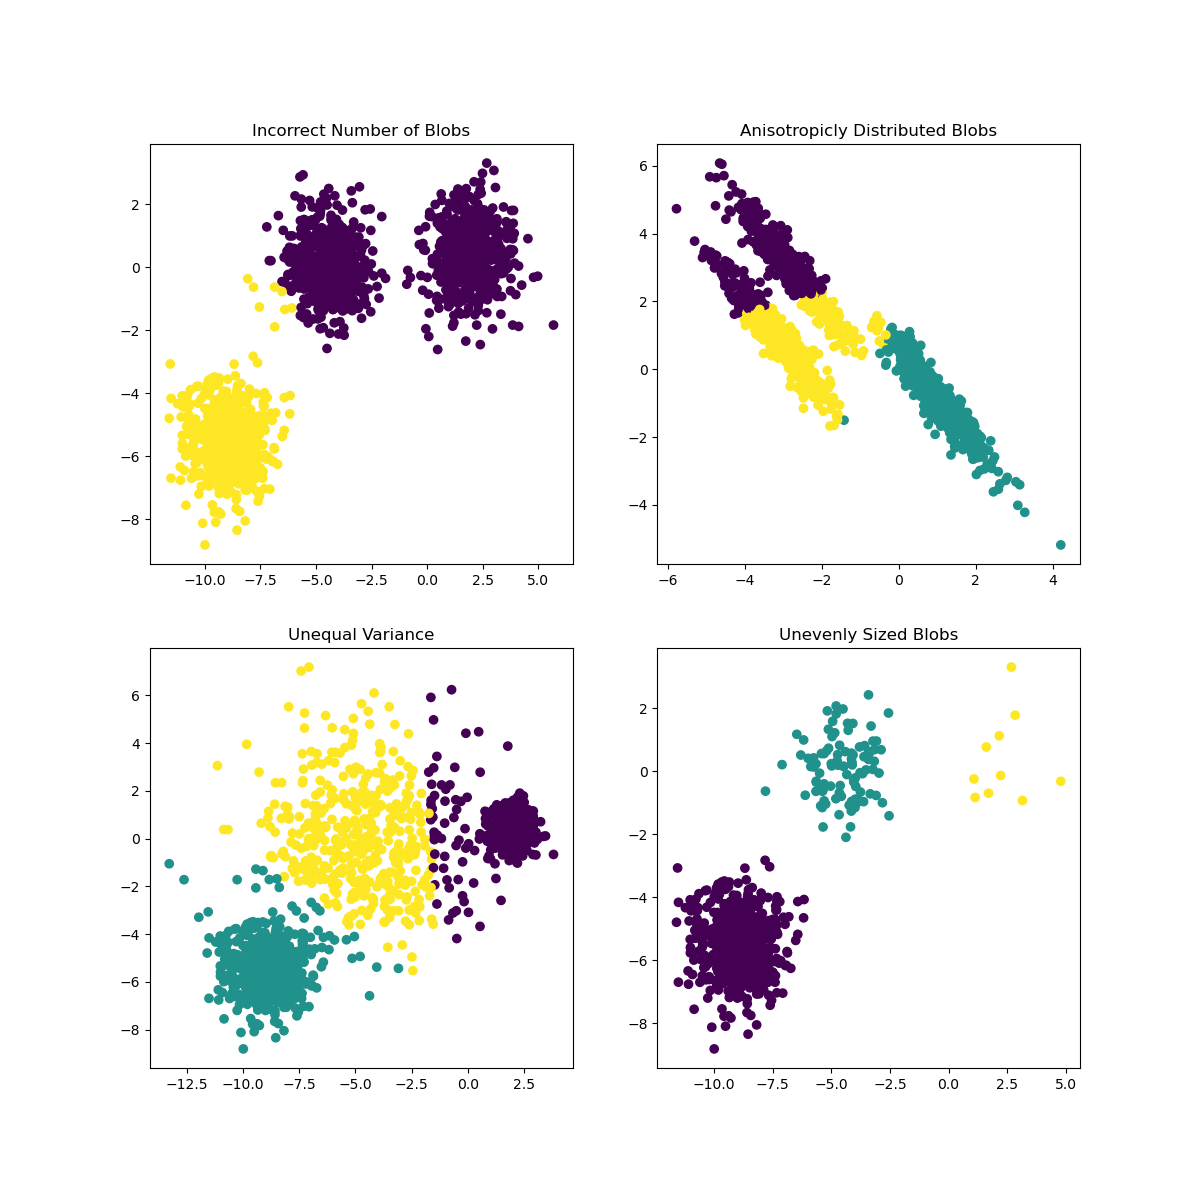
\includegraphics[height=0.9\textheight]{./resources/scikit_learn.png}
     \end{center}
\end{column}
\end{columns}
\end{frame}

\begin{frame}{Why Bother?}
\begin{itemize}
\item May want to categorize data into distinct groups by similar characteristics
\begin{itemize}
\item High growth firms; ``Cash-Cows'', etc.
\item Healthy v. Unhealthy, Kids v. Adult Cereals, etc.
\item But groups may not be interpretable..
\end{itemize}
\item Predicting with the group mean has very low variance (probably too low).
\end{itemize}
\end{frame}


\begin{frame}{Grouped Fixed Effects: Bonhomme, Lamadon, Manresa (2021) }
Wages: $W_{it}$ and $Y_{it}$: Labor Force Participation $\{0,1\}$.
\begin{align*}
Y_{i t} &=\mathbf{1}\left\{u\left(\alpha_{i 0}\right) \geq c\left(Y_{i, t-1} ; \theta_{0}\right)+U_{i t}\right\} \\
W_{i t}^{*} &=\alpha_{i 0}+V_{i t} \\
W_{i t} &=Y_{i t} \cdot W_{i t}^{*}
\end{align*}
\begin{itemize}
\item conventional FE estimator would treat $\alpha_{i0}$ and $u(\alpha_{i0})$ as unrelated parameters
\item so the FE estimate of $\theta$ would be solely based on the binary participation decisions.
\item Instead assign a common $\alpha_{i0}$ to individuals with similar $W_{it},Y_{it}$ vectors.
\end{itemize}
\end{frame}


\begin{frame}{Grouped Fixed Effects: What's the point? }
\begin{itemize}
\item Large class of models looking at matched employer-worker data.
\item Do high FE workers match to high or low FE firms?
\item Goal is often to disentangle firm FE from worker FE.
\item But workers don't change firms very often and often absorbed into firm FE.
\begin{itemize}
\item only switchers allow identification
\end{itemize}
\item See:
\begin{itemize}
\item Abowd, Kramarz and Margolis (1999): estimate full FE
\item Card, Heining and Kline (2013): bin workers by quartile of wages.
\item Bonhomme, Lamadon, Manresa (2019): grouped FE.
\end{itemize}
\end{itemize}
\end{frame}

\begin{frame}{Matched Firm/Worker Example}
\begin{align*}
Y_{i t}=a_{t}\left(k_{i t}\right)+b_{t}\left(k_{i t}\right) \alpha_{i}+X_{i t}^{\prime} c_{t}+\varepsilon_{i t}
\end{align*}
\begin{itemize}
\item Worker FE $\alpha_{i}$ drawn from distribution that depends on firm type $k_{it}$
\item Wages $Y_{it}$ drawn from distribution that depends on $\alpha_i$ and $X_{it}$ as well as firm type $k_{it}$
\item Using $k$-means:
\begin{itemize}
\item Assign firms to clusters $K=10$ based on CDF of log earnings.
\item Assign workers to $L=6$ discrete types.
\end{itemize}
\end{itemize}
\end{frame}


\begin{frame}{Grouped FE results}
\centering
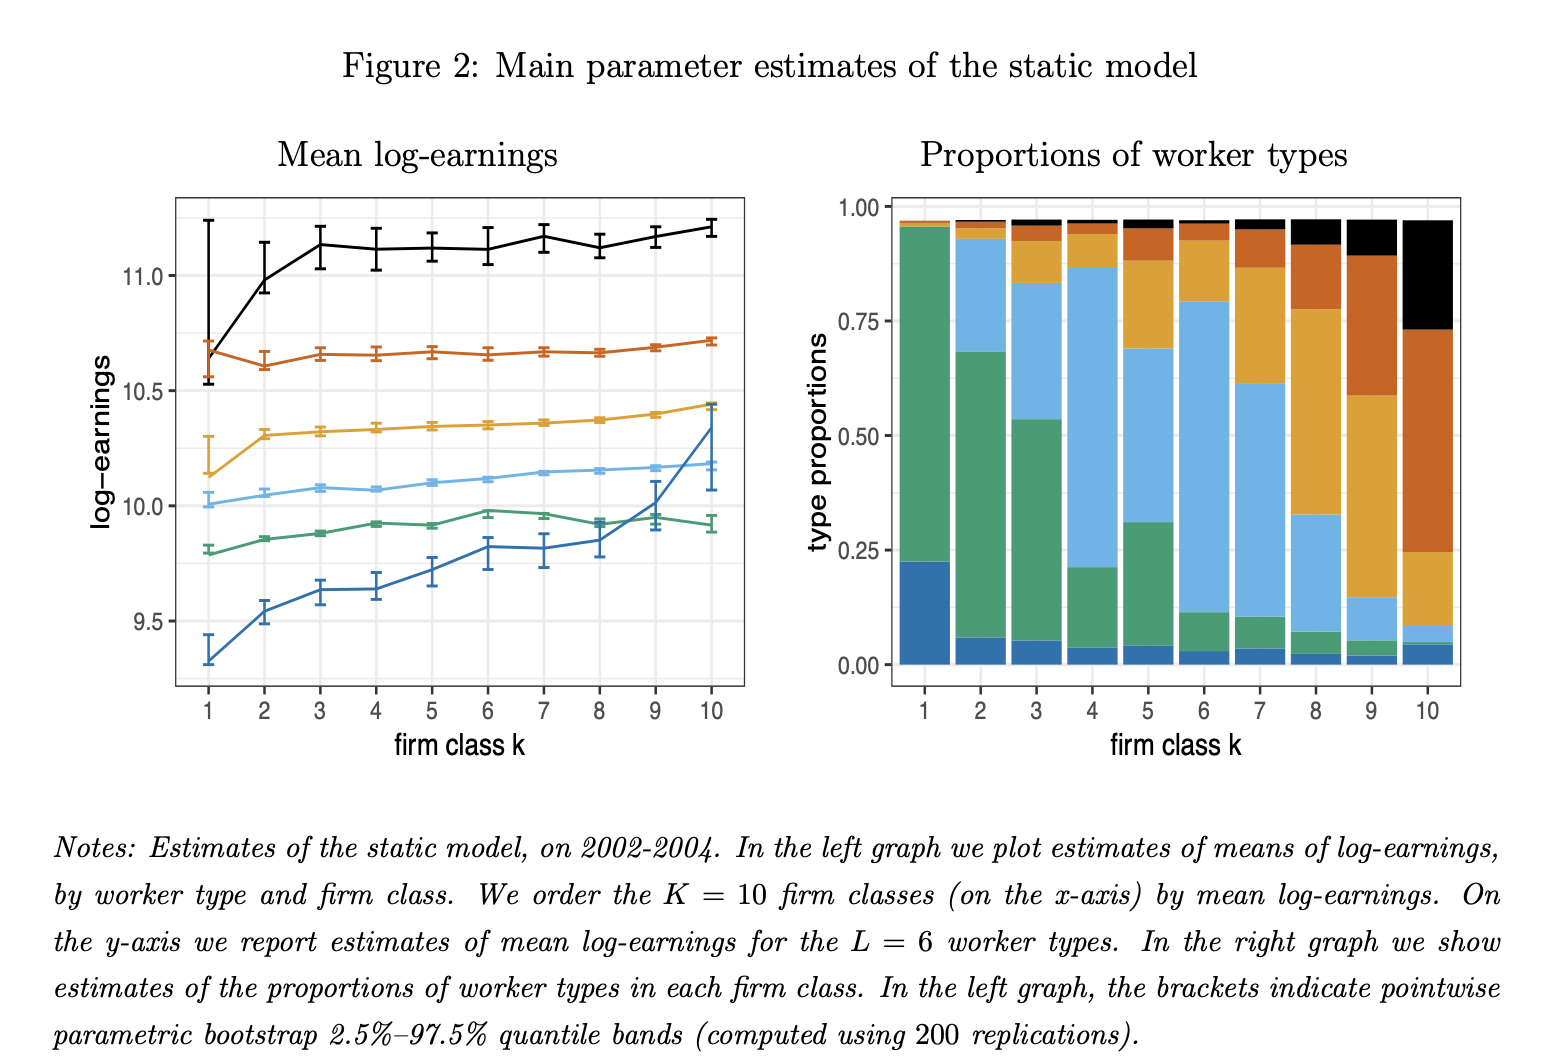
\includegraphics[height=0.9\textheight]{./resources/grouped_fe1.png}
\end{frame}


\begin{frame}{Grouped FE results}
\centering
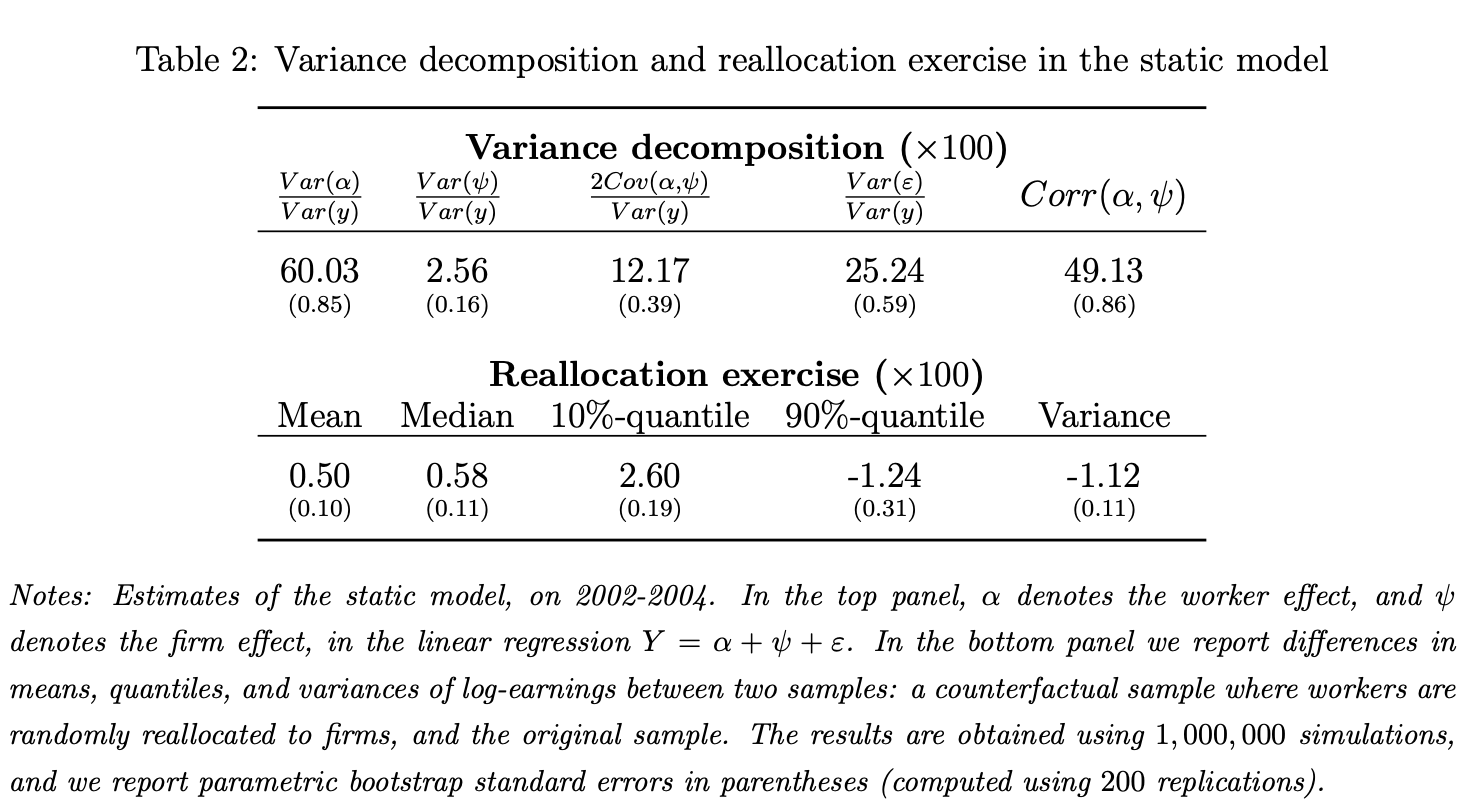
\includegraphics[height=0.9\textheight]{./resources/grouped_fe_table.png}
\end{frame}


\section{Thanks!}


\end{document}
